\chapter{Background}
The system is split into three different parts, the website, raspberry pi and the cloud(Azure), these are also split in their respective parts with website containing the web server(node) and the site(React), the Cloud; 
\begin{itemize}
  \item Azure sql server
  \item Azure sql database
\end{itemize}
\section{Website}
A website is often confused with a webpage or a web server. From mozillaWebDoc, A website is a collection of web pages which are grouped together in various ways. A web server is a computer that hosts websites and their supporting files, which are available on that computer. From a web developer point of view the webpages are known as the clients while the web servers are known as the servers. The clients are copies downloaded from the server


\subsection{Communication between clients and servers}
\begin{itemize}
  \item \textbf{Internet Connection}: This enables the transmission of data between clients and server
  \item \textbf{TCP/IP}: these are communication protocols that define how data should be transmitted on the internet. IP handles the delivery of packets of information from source to destination, TCP handles the management of these packets by joining them together in their righ t order and also asks for missing packets to be resent, this retransmission causes latency. 
  \item \textbf{HTTP}: an application layer protocol that determines how clients and server communicate.
\end{itemize}

A website talks to the web server using an API, which is a connection between to computer programs. It could be referred also as the specification or as the implementation, the specification has to do with a document that demonstrates how to use or create a connection. Examples of API specifications used in this project are; tedious for the database connection to azure, express as a middleware. 
\newacronym{HTTP}{$HTTP$}{Hypertext Tranfer Protocol}
\glsadd{HTTP}
\newacronym{TCP}{$TCP$}{transmission Control Protocol}
\glsadd{TCP}

\newacronym{API}{$API$}{Application Programming Interface}
\glsadd{API}

\section{Raspberry-pi}
A portable computer with 40 GPIO pins, 
GPIO is an uncommitted digital pin on an electronic circuit board which may be used as input or output or both, and can be configured by the user at runtime[6]. This GPIO allows to interface with different modules. A module here is a small unit that can be integrated into a larger system but also maintained separately with no effect on the system. It is of a "plug-in" functionality.
To connect to azure from the raspberry pi, "pyodbc" driver is used. The driver files are installed on the raspberry-pi
LED  

\newacronym{GPIO}{$GPIO$}{General Purpose Input Output}
\glsadd{GPIO}

\subsection{RFID - RC522}
\subsubsection{Interfacing with the Rasberry pi}
The RFID card interfaces with the raspberry-pi with SPI communication but is also compatible with 1\textsuperscript{2}C and UART communication, it is a synchronous serial communication that encourages communication over a short distance, it is mainly used in embedded systems. Serial communication has to do with sending one bit at a time sequentially and synchronous means that this communication is synchronized by a clock signal which is used orchestrate the actions of the digital circuit i.e to determine when it is time to read the next bit/value. SPI devices communicate in a full duplex mode with a master-slave principle normally with a single master. full duplex means that data is transmitted back and forth simultaneously in this communication channel.

\textit{Note: The master is the raspberry pi.}
\vspace{1cm}
\begin{figure}[h]
  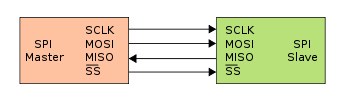
\includegraphics{Background/images/350px-SPI_single_slave.svg.png.png}
  \caption{SPI master slave architecture}
\end{figure}

\newacronym{12C}{$12C$}{Inter-Integrated Circuit}
\glsadd{12C}
\newacronym{SPI}{$SPI$}{Serial Peripheral Interface}
\glsadd{SPI}
SPI has four main logic signals: 
\begin{itemize}
  \item SCLK: Serial clock, which accepts pulses obtained from the master
  \item MOSI: Master Out Slave In, this is data transmitted from the master to slave
  \item MISO: Master In Slave Out, this is data transmitted from the slave to master
  \item CS/SS: Chip/Slave Select, an output from the master to notify data is being transmitted.
\end{itemize}

The RC522 module has 8 pins that interfaces with the raspberry pi;
\begin{itemize}
  \item SDA: 1\textsuperscript{2}C-bus serial data line input/output, it acts as as signal input when used for SPI communication
  \item SCK: SPI serial clock input which has the same operation as SCLK
  \item RST: an input for Reset and power-down of the module. It can turn off all the input pins and internal current sinks. 
  \item GND: for ground connection to the GPIO pin of the master
  \item IRQ: an interruption pin, that could notify the master when an RFID tag comes into the range of scan.
  \item 3.3v/VCC: which powers the RC522 module
  \item MOSI: has the same operation as MISO in SPI communication, receives data from master
  \item MISO: has the same operation as MOSI in SPI communication, sends data to master(raspberry pi)
\end{itemize}

\subsubsection{Operations of RFID module}
RFID tags are classified by their frequencies, the four primary frequency ranges are:
\begin{itemize}
  \item Low frequency (LF): they are frequencies from 30 to 300KHz
  \item High frequency (HF): frequencies are from 3 to 30MHz, has a higher memory size and a longer range of transmission
  \item Ultra high frequency (UHF): frequencies are from 300MHz to 3GHz
  \item Microwave frequency (microwave): they function at 2.45GHz 
\end{itemize}

\newacronym{PCD}{$PCD$}{Proximity coupling device}
\glsadd{PCD}

\newacronym{PICC}{$PICC$}{Proximity Integrated circuit card}
\glsadd{PICC}
The system consists of two main components, a transponder/tag and a transceiver/reader or a PCD and a PICC as defined in ISO 14443. The transceiver creates a 13.56MHz electromagnetic field that communicates with the tag. 
This project uses a High Frequency passive card with Type A communication defined in ISO-14443, passive meaning, the tags only function when they acquire signals from a reader and relay an information-carrying signal back to the reader. 




The rfid has a uniqueID
RFID uses electromagnetic fields to detect 




\subsection{Fingerprint - JM-101}
The JM-101 comes with a flash memory to store the fingerprints, it has a storage capacity of over. 
\subsubsection{Interfacing with Raspberry pi}
The Fingerprint interfaces with the Raspberry pi with UART communication, it is a devices that supports asynchronous serial communication, which is a form of serial communication that doesn't require a clock signal and is not constantly synchronized. Raspberry pi supports asynchronous communication but with a lot of fingerprints having distinct voltages, I used a USB to UART Converter which supports both 3.3v and 5v although the JM-101 is 3.3v. The TX pin goes to RX pin and vice versa in the connection between the converter and fingerprint module. The USB to UART Converter goes into the USB port of the raspberry pi while its pins are connected to the pins of the fingerprint module.
The pins used in interfacing with the UART converter are:
\begin{itemize}
  \item GND: ground connection
  \item RXD: the receiver of data
  \item TXD: transmits data
  \item 3V3: powers the fingerprint module
\end{itemize}

\subsubsection{Operations of fingerprint module}
Fingerprint processing can either be for enrollment or matching,  
A matching algorithm is used to compare fingerprint templates stored in the flash memory with the one read by the fingerprint module. For the 

\newacronym{UART}{$UART$}{Universal Asynchronous Receiver-Transmitter}
\glsadd{UART}

\subsection{Flask}


\subsection{Virtual tunnel}



\section{Cloud - Azure}
AzureSQL server hosts the SQL database and handles connection to other devices, programs or services. 
My options where NoSQL("Not Only SQL") or SQL also known as Sequel.
SQL is a programming language used to manage data in a relational database, I specifically used T-SQL for querying data in Microsoft SQL Server. 

\newacronym{SQL}{$SQL$}{Structured Query Language}
\glsadd{SQL}



